\documentclass[../../main.tex]{subfiles}
    
    \lstset{basicstyle=\small,
      showstringspaces=false,
      commentstyle=\color{black},
      keywordstyle=\color{blue}
    }

    \graphicspath{{../../images/Vision/}}

    \begin{document}
    \subsection{Vision}
    Wie im vorherigen Kapitel erläutert bauen viel Lösungskonzepte im Bereich
    der Objekterkennung auf der Disziplin Informatik auf. Hierbei wird immer eine Kamera
    verwendet um Informationen zu erhalten. Die Verarbeitung der Informationen und 
    schlussendlich die Objekterkennung erfolgt softwaretechnisch. Abbildung \ref{fig:vision_ablauf} 
    zeigt den prinzipieller Ablauf einer Bildverarbeitung inklusiver Featureerkennung.\\

    \begin{figure}[H] %Ablaufdiagramm Vision
        \centering
        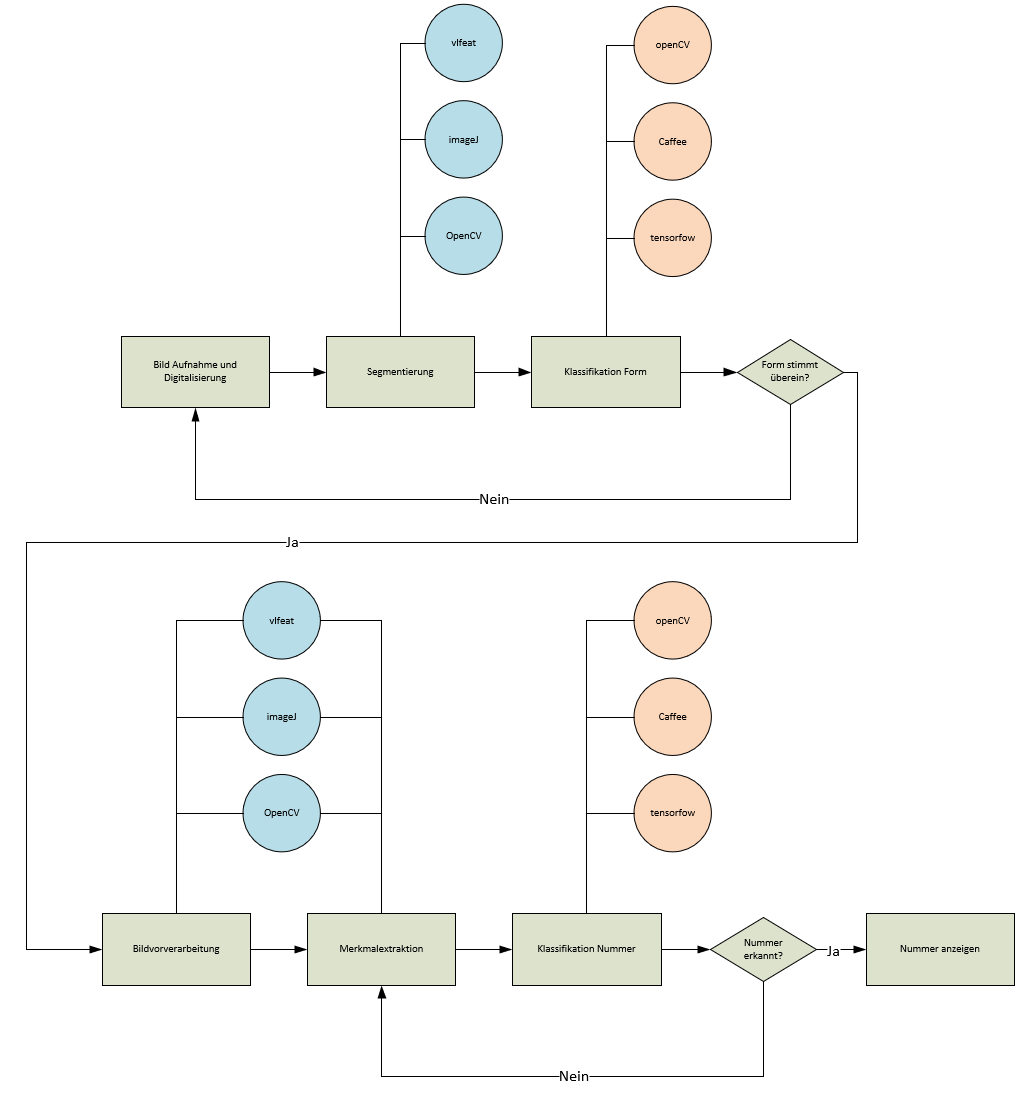
\includegraphics[width=0.8\textwidth]{Ablauf_vision.png}
        \caption{Ablaufdiagram Objekterkennung mittels Software}
        \label{fig:vision_ablauf}
    \end{figure}
    
    
    
    
    
    \end{document}
